% --- CHAPTER 1: CONCEPT ---
\section{Concept and Architectural Foundation}
\label{sec:concept}

This report presents the architectural specification and system validation of \textbf{AdriaBOX}, an enterprise-grade, multi-tenant distributed object storage matrix engineered to provide fault-tolerant, highly available, and cryptographically isolated asset persistence over a cluster of independent storage nodes. AdriaBOX addresses the structural design and performance limits inherent in legacy file systems by applying a strict separation of concerns across a multi-component topology.

\subsection{System Classification and Decoupled Architecture}
Architecturally, AdriaBOX is implemented as a highly decoupled, heterogeneous computing infrastructure. The entire platform is partitioned into two distinct functional operating horizons, separating the control pathways from high-throughput binary transmission lines:
\begin{itemize}
    \item \textbf{The Control Plane (Orchestration Core):} Represented by a centralized Metadata Controller running as an asynchronous, stateful Web-service backed by the Flask framework. The control plane acts as the authoritative source of truth for the cluster, exposing RESTful endpoints tasked exclusively with tenant session authentication, cryptographic token issuance, relational storage planning, and real-time node telemetry auditing.
    \item \textbf{The Data Plane (Decentralized Worker Fleet):} Composed of a horizontal fleet of autonomous, multi-threaded background storage node daemons. These daemons are bound to independent network interfaces and task-isolated storage partitions, operating as low-level binary engines optimized for raw byte extraction and synchronous pipeline replication cascade enforcement.
\end{itemize}

The global operational boundary, network plane isolation, and multi-tier component distribution are formalized in the infrastructure blueprint detailed in \Cref{fig:architectural_decoupling}.

\begin{figure}[htbp]
    \centering
    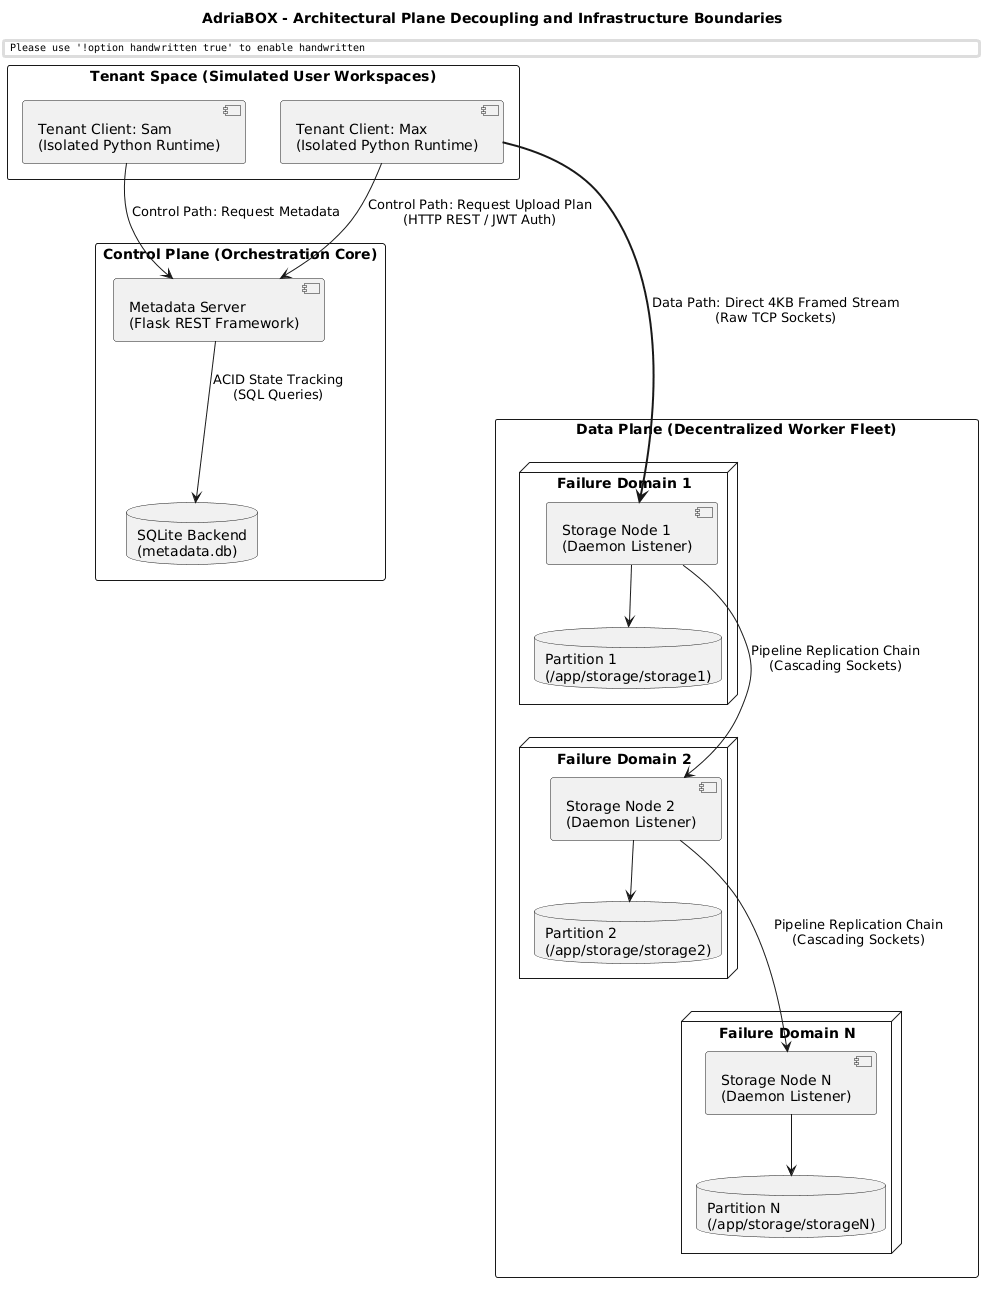
\includegraphics[width=0.85\textwidth]{plantuml/1.1-architectural-decoupling.png}
    \caption{AdriaBOX Architectural Plane Decoupling and Infrastructure Plane Separation Boundary.}
    \label{fig:architectural_decoupling}
\end{figure}

The transition from procedural, monolithic paradigms—typical of legacy software frameworks written in standard C—into an object-oriented Python architecture is driven by the necessity to implement clean component abstraction barriers. Python 3.14 provides native support for structured class inheritance, robust error trapping, and state virtualization facades. This choice allows the platform to encapsulate complex network socket streams and multi-layered database transactions inside highly maintainable object interfaces, while maintaining complete access to underlying system-level calls.

\subsection{The Object Storage Paradigm and Flat Namespace Mathematics}
Unlike traditional centralized distributed file systems that recursively map directory layouts as logical structural trees using parent-child relational references, AdriaBOX adopts an \textbf{Object Storage Flat Namespace} paradigm. Within the storage nodes and the centralized database tracking maps, directories do not exist as physical or logical entities. Folders are instead abstracted as virtual textual string prefixes integrated directly into the object identifier keys. For example, a file visualized by the client interface as residing within a multi-tiered folder hierarchy is recorded globally as a single string key token:
$$\text{Object Key Index: } K = \text{``/documents/pizzeria/file\_example.avi''}$$

The absolute structural benefits of this design choice become clear when evaluating the temporal complexity of global metadata operations. In a standard filesystem, renaming a directory or moving a branch containing thousands of deeply nested files requires a blocking execution loop to recursively traverse relational keys or manipulate physical disk blocks. In AdriaBOX, because paths are merely string key properties within a relational matrix, actions like folder creation (\texttt{mkdir}) or directory prefix migration (\texttt{mv}) achieve an execution temporal efficiency of exactly $O(1)$ complexity. Modifying an entire namespace section is instantaneous and non-blocking; it is executed via a single, atomic SQL update statement targeting matching string prefix patterns on the control plane database, completely bypassing any data repositioning across the storage cluster. This mapping layout is formalized in \Cref{fig:flat_namespace}.

\begin{figure}[htbp]
    \centering
    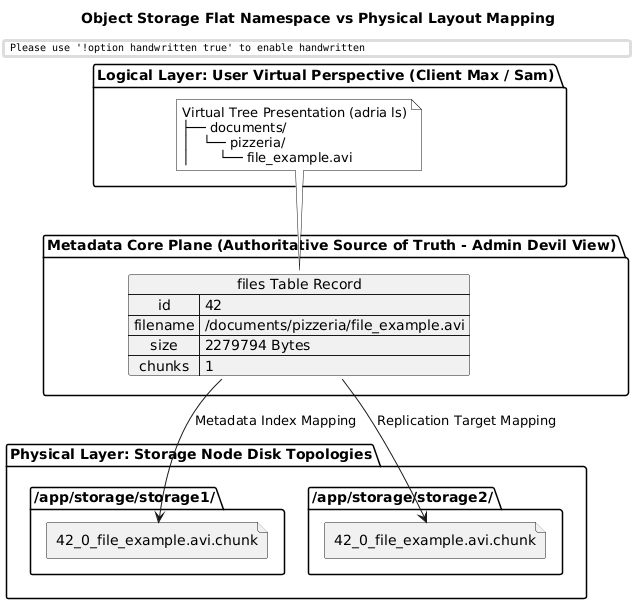
\includegraphics[width=0.9\textwidth]{plantuml/1.2-flat-namespace.png}
    \caption{AdriaBOX Object Storage Flat Namespace Mapping Blueprint vs Physical Disconnected Topologies.}
    \label{fig:flat_namespace}
\end{figure}

\subsection{Structural Slicing and Data Plane Virtualization}
To manage massive file storage allocation without creating unbalanced workloads or hitting volume capacity barriers on individual worker machines, the control plane enforces automated binary file striping. When a user initiates an upload transaction, the metadata controller evaluates the global asset capacity in bytes. If the asset scale surpasses the maximum logical partition threshold defined within the system configuration constants ($LOGICAL\_BLOCK\_SIZE = 64$ Megabytes), the file object is mathematically sliced into separate, autonomous logical fragments. Each block is tracked via a deterministic allocation matrix using a specialized ceiling function:
$$N = \max\left(1, \left\lceil \frac{\text{File Size}}{64 \times 1024 \times 1024} \right\rceil\right)$$

The individual data blocks are assigned unique, structured names based on their file ID and chunk index (e.g., \texttt{42\_0\_file.chunk}, \texttt{42\_1\_file.chunk}), and are then distributed across the storage node fleet. The worker daemons virtualize physical storage by isolating these incoming blocks within dedicated host directories. Each background process is jailed inside a specific container partition path (ranging from \texttt{/app/storage/storage1} to \texttt{/app/storage/storage12}), effectively simulating twelve disconnected, independent hardware failure domains on the host system.

\subsection{Use Case Specification and Multi-Tenant Role Demarcation}
AdriaBOX is engineered from the ground up for multi-tenant deployment across shared enterprise or academic intranet networks. The platform isolates user spaces by strictly separating administrative capabilities from standard user operations. While designed to deploy across physically distinct client stations, the validation environment emulates multi-tenant concurrency by deploying isolated concurrent workspaces. This layout isolates active session variables and Zero-Knowledge security frames inside segregated user contexts, ensuring that different active clients cannot contaminate shared storage boundaries or intercept keys.
\begin{itemize}
    \item \textbf{Standard Tenant (User Role):} Authorized to execute standard data manipulation routines within their isolated account context. Users can create virtual directory prefixes, upload new assets, download or permanently delete existing files, and check their individual storage quota allocation metrics. A standard user has zero visibility into the identities, quotas, or metadata blocks of other registered tenants.
    \item \textbf{System Administrator (Admin Role):} Authorized to audit and manage the cluster infrastructure. System administrators can query real-time node heartbeats, evaluate aggregate cluster footprints, and execute cascading user evictions. However, due to client-side cryptographic barriers, administrators are prevented from reading the raw binary contents of tenant files.
\end{itemize}

The global system interaction framework is transaction-bound and event-driven. The client application remains completely passive until a user invokes a command via the CLI terminal. In contrast, the metadata master and decentralized storage node processes run continuously as non-blocking system services, listening for network connections on their designated interface ports.

\subsection{The Necessity of Distribution and Resource Isolation}
Designing AdriaBOX as a decentralized storage matrix rather than a traditional centralized server application resolves critical architectural bottlenecks in resource management, data availability, and network scalability:

\begin{enumerate}
    \item \textbf{Data Path Offloading and Bandwidth Optimization:} In centralized storage designs, all binary data streams must pass directly through the central server's network interface card, creating extreme performance bottlenecks as user concurrency increases. AdriaBOX completely eliminates this issue by removing the Metadata Server from the data transfer path. The master node only processes lightweight, sub-millisecond REST control messages to generate or validate storage roadmaps. High-throughput binary streaming is delegated entirely to parallel peer-to-peer TCP channels opened directly between the client CLI and specific storage nodes.
    \item \textbf{Fault Domain Isolation and Synchronous Survival Chains:} Hardware failure is a certainty in large-scale cluster environments. AdriaBOX mitigates this risk by mirroring each logical block across three unique failure domains via a synchronous replication cascade. If an individual storage node crashes or suffers a sudden disk failure, data availability is maintained with zero downtime by shifting transactions to one of the remaining online replica copies.
    \item \textbf{Resource Starvation Mitigation ($O(1)$ Memory Page Safety):} A major vulnerability in cloud storage software is the tendency to load entire chunks or files into central memory (RAM) via blocking operations, which triggers kernel out-of-memory (OOM) panics during large file upload streams. AdriaBOX guarantees absolute memory safety by enforcing a strict buffered streaming model. By mapping the application data transfer page to a fixed size configuration ($CHUNK\_SIZE = 4096$ Bytes)—aligning with the native physical memory page allocation of standard Linux kernels—the client and worker engines move binary data through a continuous stream of micro-packets. During high-concurrency binary uploads, this model avoids memory leaks or process context interference, keeping the active RAM footprint strictly bounded at exactly 4 Kilobytes regardless of whether the target asset is a lightweight document or a multi-gigabyte archive.
\end{enumerate}